\documentclass[11pt]{article}
\usepackage[margin=1in]{geometry}
\usepackage{booktabs,graphicx,amsmath,amssymb,microtype,xcolor}
\usepackage[hidelinks]{hyperref}
\usepackage{caption}
\captionsetup{font=small,labelfont=bf}
\newcommand{\code}[1]{\texttt{\small #1}}

\title{\textbf{Lifetime Integrity:\\Short-Horizon Evaluation Misranks Persistent-State Maintenance Policies}}
\author{in-c0}
\date{2026-09-04 --- working draft}

\begin{document}
\maketitle

\begin{abstract}
Persistent agents accumulate stale, contradictory, and superseded information
over long deployments. That agents degrade this way is established. What is not
established is whether the \emph{maintenance policies} used to counter it retain
their relative merit as lifetimes lengthen, once the evidence access they consume
is explicitly metered. We introduce LIS-v0, an architecture-agnostic benchmark in
which a locked corruption process --- contradictions, misinformation, misleading
repetition, genuine world change, inactivity gaps, context shifts, and unequal
source reliability --- is held fixed while \emph{lifetime length is the
independent variable}, and every historical evidence access is charged against an
enforced, equal ceiling. We evaluate nine maintenance policies over 12 paired
preregistered seeds at horizons $\{8,16,32,64,128\}$. Three findings follow.
First, mechanism rankings are strongly horizon-dependent: the mean Spearman
correlation between rankings at 8 and 128 epochs is $\rho = 0.335$
(95\% CI $[0.252, 0.415]$), with all 12 seeds below the preregistered threshold
of $0.6$ --- short-horizon evaluation is unsafe for selecting maintenance
policies. Second, cost buys little integrity: at 128 epochs the Pareto frontier
is occupied by a zero-read decay heuristic and a periodic reset costing 1.7\% of
the read ceiling, while reliability-weighted re-grounding spends 245{,}347 reads
and is \emph{worse} than the free heuristic. Third, correctness and integrity are
not interchangeable: two policies statistically indistinguishable in accuracy
differ measurably in integrity violation. A second experiment on ambiguous
delayed blame yields a deliberately awkward negative result: a policy can show a
positive causal contrast against inaction while both it and the baseline are
degrading, and its ability to repair the responsible belief reverses with
horizon. We claim no result about any learned latent substrate.
\end{abstract}

\section{Introduction}
\label{sec:intro}

A deployed agent that keeps state does not merely answer questions; it carries
beliefs forward. Over a long enough deployment those beliefs meet contradiction,
misinformation, genuine change in the world, and long silences. That such systems
degrade is no longer in question and has been documented across deployment
lifespans, stale-memory detection, and belief drift
(\S\ref{sec:related}).

The question this paper asks is narrower and, we argue, more actionable. Suppose
you must \emph{choose} a maintenance policy. You benchmark several over a
plausible interaction length, pick the winner, and deploy. Is that choice stable?
And when a policy earns its ranking by re-reading history, is the integrity it
buys worth what it spends?

Both questions require two things absent from existing evaluations: a corruption
process held \emph{fixed} across the compared policies, and resource accounting
that is \emph{enforced} rather than reported. We provide both, and add lifetime
length as an explicit independent variable.

\paragraph{Contributions.}
\begin{enumerate}\itemsep2pt
\item \textbf{LIS-v0}, an architecture-agnostic benchmark with a locked corruption
      process, a metered evidence log with an enforced equal read ceiling, and
      integrity metrics that can disagree with correctness.
\item \textbf{Evidence that short-horizon evaluation misranks policies}:
      $\rho = 0.335$ between 8- and 128-epoch rankings across 12 preregistered
      seeds, all below the frozen $0.6$ threshold.
\item \textbf{A cost result}: expensive re-grounding does not purchase
      proportionate long-horizon integrity on LIS-v0; the frontier is held by
      free and near-free policies.
\item \textbf{A negative result on ambiguous delayed blame}, including the
      distinction between a positive causal contrast and actual repair.
\item \textbf{A fully sealed protocol}: preregistration, amendment history,
      frozen seeds, and every table and figure regenerable from committed
      manifests.
\end{enumerate}

\section{Related work and novelty boundary}
\label{sec:related}

This work sits in a crowded area, and we state plainly what we do not claim.
Our literature audit was refreshed immediately before the confirmatory freeze;
every record below was verified against its primary arXiv entry rather than a
search summary.

\paragraph{We claim no novelty for} persistent-agent aging or degradation
(AgingBench, arXiv:2605.26302); stale-memory detection (STALE, arXiv:2605.06527);
belief drift and evidence-driven revision across sessions (BeliefShift,
arXiv:2603.23848); contradiction resolution with bitemporal provenance (TOKI,
arXiv:2606.06240) or transactional belief commit with cascading repair (MemTX,
arXiv:2607.23929); provenance-capped, reliability-conditional belief updating
(arXiv:2606.22030); offline or sleep-style consolidation and replay
(arXiv:2606.03979, arXiv:2604.20943); hindsight credit assignment to
memory-writing actions (HiMPO, arXiv:2606.16285); collateral-damage measurement
after targeted edits (RippleEdits, arXiv:2307.12976; MQuAKE, arXiv:2305.14795);
closed-world symbolic belief benchmarks with exact turn-level scoring
(BeliefTrack, arXiv:2605.30219); or the term \emph{epistemic integrity} for
long-running agents (arXiv:2606.04017).

\paragraph{Three near neighbours require precise separation.}
\emph{Maintenance cost} is already studied: arXiv:2606.24775 evaluates twelve
memory systems and reports that localized maintenance is more cost-efficient,
and arXiv:2606.06448 profiles agent-memory cost across construction, retrieval
and generation. Neither enforces an equal metered ceiling across compared
policies, nor holds a locked corruption process fixed; both compare whole
\emph{systems} on natural workloads rather than \emph{policies} at parity.
\emph{Long horizons} are already studied: AMA-Bench (arXiv:2602.22769) scales to
arbitrary horizons and AgingBench spans 8--200 sessions. Neither uses horizon to
test whether the \emph{ranking} of mechanisms is stable. \emph{Grounding
separated from correctness} already exists: EvidenceRL (arXiv:2603.19532) scores
entailment with retrieved evidence separately from answer agreement, but for
single-turn retrieval-augmented responses, not for persistent state accumulated
across a lifetime; SAVeR (arXiv:2604.08401) motivates itself on unsupported
beliefs but audits within a trajectory before commitment.

\paragraph{Residual contribution.} Not any one of these ingredients, but their
conjunction: a locked corruption process, an enforced and reported maintenance
cost, lifetime length as an experimental independent variable, integrity metrics
that can disagree with correctness, and paired evaluation of persistent
maintenance policies. For ambiguous delayed blame with collateral scoring
(\S\ref{sec:b001}) we found no direct precedent --- ReBel (arXiv:2605.20061)
frames delayed reward as obscuring which intermediate belief was at fault but is
a policy-optimization method without ambiguous multi-belief attribution or
collateral measurement --- and our result there is negative.

\section{The Lifetime Integrity benchmark}
\label{sec:benchmark}

\begin{figure}[t]\centering
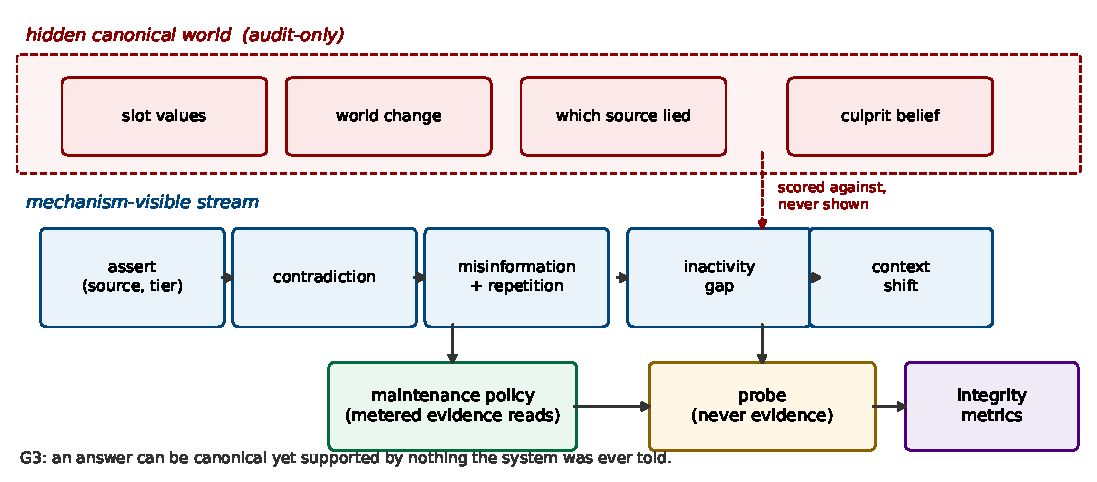
\includegraphics[width=\textwidth]{figures/fig1_concept.pdf}
\caption{One interrupted lifetime in LIS-v0. A hidden canonical world generates a
mechanism-visible stream of assertions, contradictions, misinformation with
misleading repetition, inactivity gaps and context shifts. The maintenance policy
sees only the visible view and reaches history through a metered evidence log.
Probes are scored against audit-only ground truth and are never available as
evidence.}
\label{fig:concept}
\end{figure}

A \emph{lifetime} is a deterministic event sequence over hidden context/key slots
drawn from a shared codebook, so that a bounded state can bleed a neighbouring
slot's value. Event types are assertions (tagged audit-only as clean,
misinformation, misleading repetition, contradiction, or world change), probes,
inactivity gaps, and context shifts. Sources belong to \emph{primary},
\emph{secondary} and \emph{unreliable} tiers with differing hidden reliability,
and some world changes are \emph{quiet}: the canonical value changes with no
announcement.

\paragraph{Audit separation.} Canonical values, truthfulness flags, corruption
tags, probe classes and superseded-value lists are harness-only. Mechanisms
receive a redacted view; the harness counts any leak and the validator rejects a
comparison with a non-zero count.

\paragraph{Integrity is not accuracy.} Two failures are invisible to a
correctness score. A system may answer the canonical value \emph{that nothing
ever told it} --- right by luck or confabulation, and ungrounded. Or it may
answer a value it was legitimately told which has since been superseded. We
therefore score \code{unsupported\_belief\_rate} (answered a value absent from
everything asserted about that slot), \code{stale\_state\_rate} (answered a
superseded value), their union \code{integrity\_violation\_rate} (IVR, the
primary endpoint), \code{self\_contradiction\_rate} (an answer flipping with no
intervening evidence) and \code{provenance\_consistency}. Abstention is never an
integrity violation.

\paragraph{Metered evidence.} Re-grounding is not free. A policy that stays
coherent by re-reading everything has not solved a problem a large enough context
window would not also solve. Historical access therefore goes through a bounded
log that charges per record \emph{scanned}, refuses reads past a shared ceiling,
and records exhaustion. This turns ``budget-matched'' from a claim into a
property the validator checks.

\section{Protocol and resource accounting}
\label{sec:protocol}

\paragraph{Phases.} Pilot (non-evidential), development calibration on three
reserved seeds, then confirmatory on twelve seeds disjoint from both. The
corruption process was locked before development and never changed.

\paragraph{Frozen quantities.} Corruption process
\code{0ebb3e60\ldots}; scoring protocol \code{LIS-SCORE-v0.3.0}
(\code{c001a916\ldots}); matched-control version
\code{matched-contemporaneous-v1}; window $k=3$; evidence-read ceiling
$\mathrm{round}(1.25 \times n_{\text{probes}} \times 200) = 2500 \times
\text{epochs}$, identical for every arm; horizons $\{8,16,32,64,128\}$; twelve
confirmatory seeds derived by a committed SHA-256 rule excluding all pilot and
development seeds.

\paragraph{Claim-scoped validity.} A structural or provenance failure invalidates
an entire cell. A metric that is inert invalidates only the claims that
\emph{depend} on it. This matters: at 8 epochs each slot receives too few probes
to form consecutive un-evidenced pairs, so \code{self\_contradiction\_rate} is
structurally near-zero and would otherwise have suppressed a hypothesis that
never consumes it.

\paragraph{Statistics.} The resampling unit is the lifetime seed; arms stay
paired within a resampled seed; horizons are analysed separately. All intervals
are percentile bootstrap with 10{,}000 replicates and a deterministic RNG derived
by SHA-256 from experiment, claim and horizon. Three primary tests were
predeclared under Holm--Bonferroni at family-wise $\alpha = 0.05$; everything
else is secondary or exploratory. We report effect sizes and intervals, and avoid
``significant'' as a synonym for important.

\paragraph{Amendment history.} Two protocol changes are part of the record. A
\emph{pre-development} measurement repair replaced a degenerate global untouched
control with matched contemporaneous controls. A \emph{post-development,
pre-confirmatory} amendment introduced claim-scoped validity, replaced the
absolute repair endpoint with a paired causal one, raised the read ceiling by a
fixed 1.25 factor (verified inert before exhaustion across all 210 development
arm-runs), and clarified matched-control semantics. Both are documented in the
repository with their motivating observations.

\section{A001: maintenance under lifetime scaling}
\label{sec:a001}

\begin{figure}[t]\centering
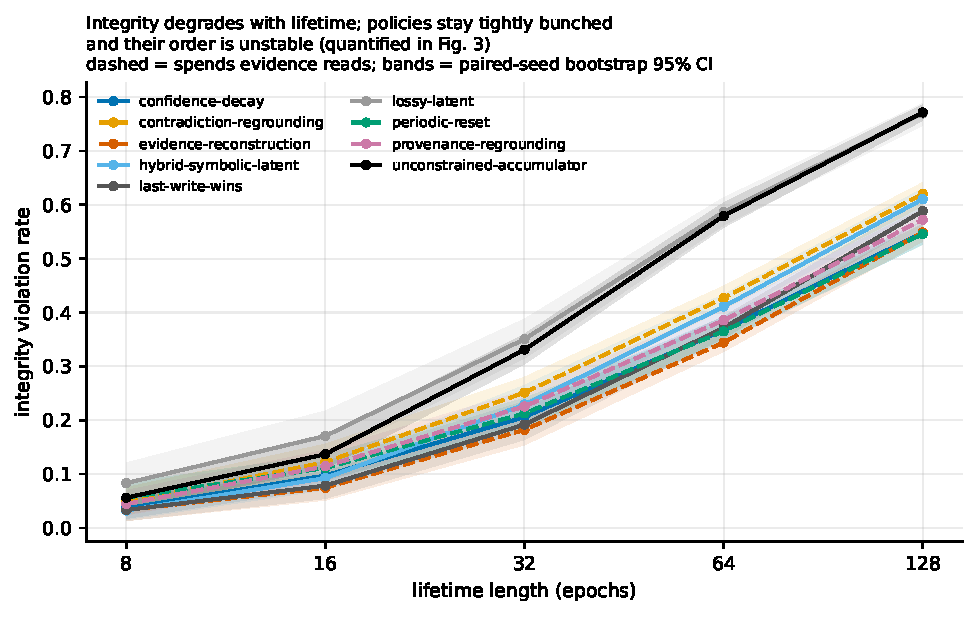
\includegraphics[width=0.86\textwidth]{figures/fig2_integrity_vs_horizon.pdf}
\caption{Integrity violation against lifetime length for all nine policies.
Bands are paired-seed bootstrap 95\% intervals; dashed lines spend evidence
reads. Curves cross repeatedly: the ordering at 8 epochs is not the ordering at
128.}
\label{fig:horizon}
\end{figure}

\begin{figure}[t]\centering
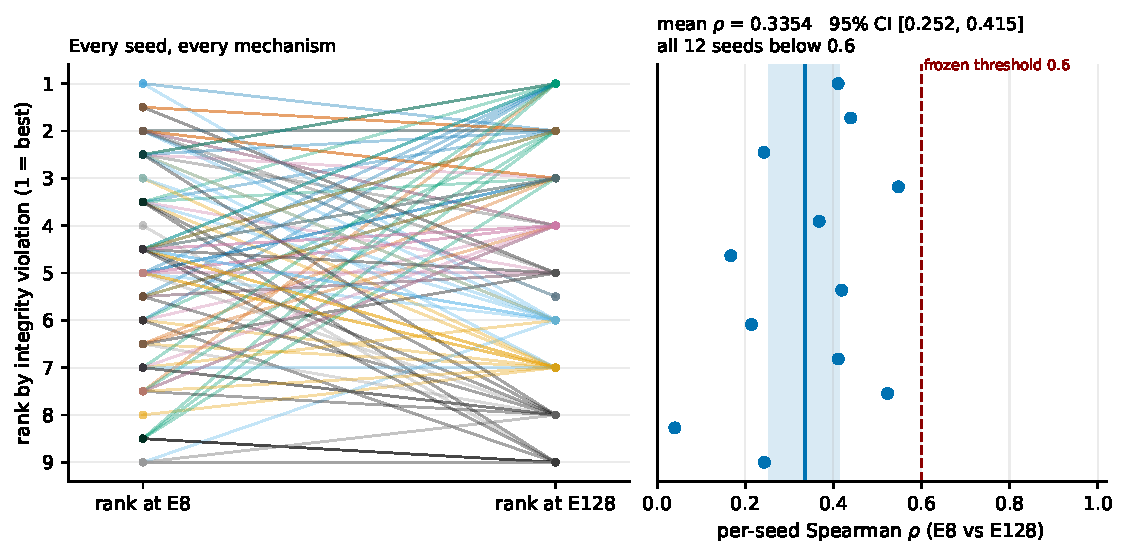
\includegraphics[width=\textwidth]{figures/fig3_rank_instability.pdf}
\caption{Left: every mechanism in every seed, ranked at 8 epochs and again at 128.
Right: the twelve per-seed Spearman correlations, their mean and bootstrap 95\%
interval, against the preregistered $0.6$ threshold.}
\label{fig:rank}
\end{figure}

\paragraph{H2: rankings do not transfer across horizons.}
The preregistered diagnostic ranks the nine mechanisms by IVR at 8 and at 128
epochs and takes the Spearman correlation per seed. The mean is
$\rho = 0.3354$, 95\% CI $[0.2517, 0.4146]$; the interval excludes $1.0$ and the
mean is below the frozen $0.6$. Every one of the twelve seeds individually falls
below the threshold, the largest being $0.548$. Beyond the binary decision, the
magnitude matters: a correlation near $0.34$ means a substantial fraction of the
ordering is rearranged between the two horizons.

\paragraph{H1: a cheap policy beats the unconstrained accumulator.}
At 128 epochs, \code{confidence-decay} attains an IVR $0.2234$ lower than the
unconstrained accumulator (95\% CI $[-0.2378, -0.2089]$) while spending
\emph{zero} evidence reads.

\begin{figure}[t]\centering
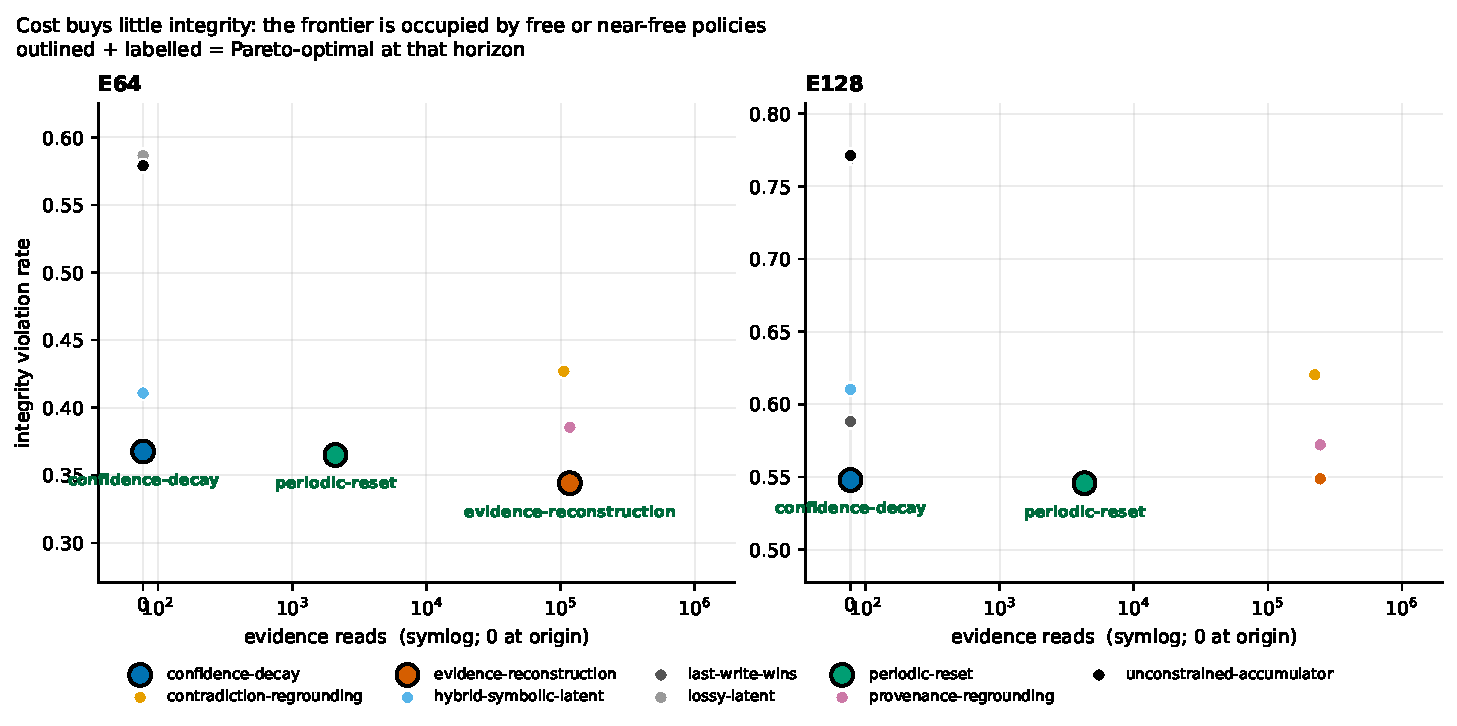
\includegraphics[width=\textwidth]{figures/fig4_cost_frontier.pdf}
\caption{Integrity against evidence reads at 64 and 128 epochs. Outlined,
labelled points are Pareto-optimal.}
\label{fig:frontier}
\end{figure}

\paragraph{The cost frontier.} Table~\ref{tab:frontier} and
Figure~\ref{fig:frontier} give the central practical result. At 128 epochs the
frontier contains \code{confidence-decay} (IVR $0.5479$, zero reads) and
\code{periodic-reset} (IVR $0.5457$, $4{,}290$ reads --- 1.7\% of the ceiling).
\code{evidence-reconstruction} and \code{provenance-regrounding} each spend
$245{,}347$ reads, 57 times \code{periodic-reset}, and neither reaches the
frontier. \code{provenance-regrounding} is \emph{worse} than the free heuristic
($0.5721$ vs.\ $0.5479$) at 96\% ceiling utilisation. Reliability-weighted
re-grounding purchases nothing here.

\begin{table}[t]\centering\small
\begin{tabular}{lrrrrrc}
\toprule
Mechanism & IVR & Accuracy & Evid. reads & Maint. ops & State bytes & Pareto \\
\midrule
periodic-reset & 0.5457 & 0.662 & 4,290 & 36 & 869 & $\bullet$ \\
confidence-decay & 0.5479 & 0.686 & 0 & 0 & 2,088 & $\bullet$ \\
evidence-reconstruction & 0.5487 & 0.672 & 245,347 & 0 & 0 &  \\
provenance-regrounding & 0.5721 & 0.711 & 245,347 & 0 & 268 &  \\
last-write-wins & 0.5882 & 0.708 & 0 & 0 & 656 &  \\
hybrid-symbolic-latent & 0.6103 & 0.749 & 0 & 0 & 3,214 &  \\
contradiction-regrounding & 0.6204 & 0.736 & 223,261 & 1,151 & 1,377 &  \\
lossy-latent & 0.7694 & 0.439 & 0 & 0 & 1,432 &  \\
unconstrained-accumulator & 0.7713 & 0.441 & 0 & 0 & 2,088 &  \\
\bottomrule
\end{tabular}
\caption{Long-horizon (E128) cost frontier, means over 12 seeds.}
\label{tab:frontier}
\end{table}

\paragraph{H3: accuracy and integrity dissociate.}
At 128 epochs exactly one pair qualifies under the preregistered criterion:
\code{last-write-wins} and \code{provenance-regrounding} are statistically
indistinguishable in canonical accuracy (difference $-0.0027$, interval spanning
zero) while differing in integrity violation ($+0.0160$, 95\% CI
$[+0.0051, +0.0270]$). One qualifying pair is thin support and we report it as
such, but it is a direct demonstration that a correctness score would have called
these two policies equivalent.

\begin{figure}[t]\centering
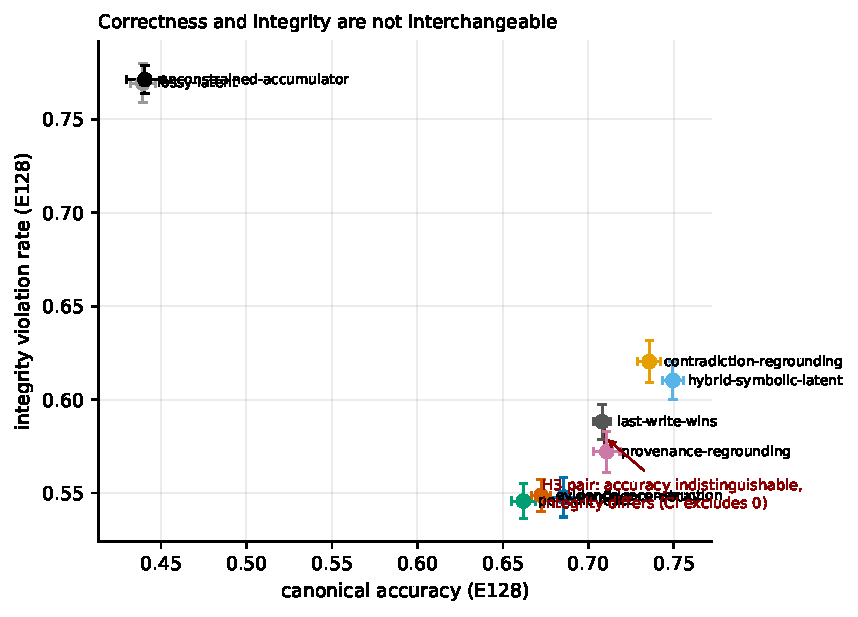
\includegraphics[width=0.66\textwidth]{figures/fig5_accuracy_vs_integrity.pdf}
\caption{Accuracy against integrity at 128 epochs. The highlighted pair is
accuracy-matched but integrity-separated.}
\label{fig:acc}
\end{figure}

\section{B001: ambiguous delayed blame}
\label{sec:b001}

A delayed outcome reports that a decision failed and names the slots it
consulted, without saying which carried the bad value. Five credit-assignment
rules share one belief substrate so that the rule is the only variable. Because
inaction itself has a non-zero, horizon-dependent effect on the measured
trajectory, the causal endpoint is
$\mathrm{excess} = \mathrm{net\_repair}(\pi) - \mathrm{net\_repair}(\text{no-consolidation})$
on the identical paired lifetime.

\begin{figure}[t]\centering
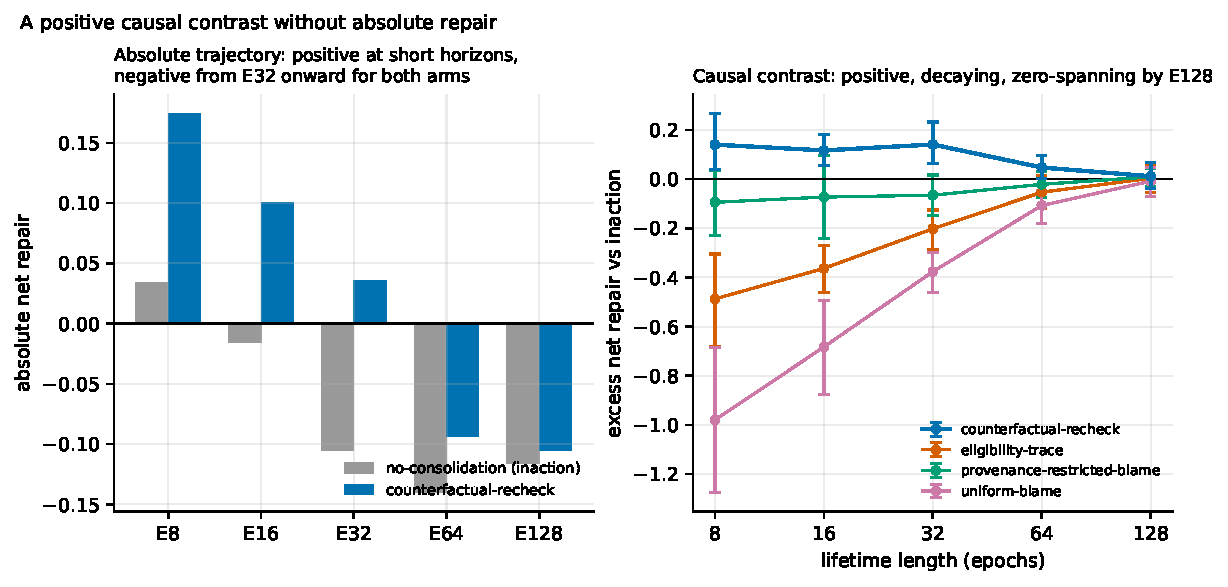
\includegraphics[width=\textwidth]{figures/fig6_b001_causal_vs_absolute.pdf}
\caption{Left: absolute net repair for the inaction baseline and the best policy.
Right: the paired causal contrast with bootstrap intervals. A positive contrast
coexists with a deteriorating absolute trajectory at long horizons.}
\label{fig:b001}
\end{figure}

\paragraph{The preregistered endpoint passes, and that is not the whole story.}
At the preregistered horizon of 64 epochs, \code{counterfactual-recheck} attains
excess $+0.0469$ (95\% CI $[+0.0032, +0.0939]$), which survives Holm correction.
But at that horizon its \emph{absolute} net repair is $-0.0933$ and the inaction
baseline is $-0.1402$: both are degrading. The culprit-specific delta is
$-0.0331$ with an interval spanning zero. At 64 epochs the policy therefore
achieves \textbf{relative mitigation --- less degradation than inaction ---
rather than demonstrated repair}.

\paragraph{Repair is horizon-dependent and reverses.}
Table~\ref{tab:culprit} traces the culprit-specific delta across horizons. At 32
epochs there \emph{is} absolute culprit repair ($+0.0659$, 95\% CI
$[+0.0152, +0.1204]$). At 64 epochs the effect is inconclusive, and at 128 epochs
the same policy significantly \emph{degrades} the responsible belief ($-0.0382$,
95\% CI $[-0.0670, -0.0042]$). These are exploratory quantities under our frozen
claim tiers and uncorrected across horizons and arms, so they cannot carry a
headline claim; we report them because omitting them would misstate the evidence.

\begin{table}[t]\centering\small
\begin{tabular}{lrrrl}
\toprule
Horizon & $n$ seeds & Culprit $\Delta$ & 95\% CI & Reading \\
\midrule
E8 & 12 & +0.1086 & [-0.1159, +0.3160] & inconclusive \\
E16 & 12 & +0.0780 & [-0.0438, +0.1895] & inconclusive \\
E32 & 12 & +0.0659 & [+0.0152, +0.1204] & absolute repair \\
E64 & 12 & -0.0331 & [-0.0852, +0.0165] & inconclusive \\
E128 & 10 & -0.0382 & [-0.0670, -0.0042] & deterioration \\
\bottomrule
\end{tabular}
\caption{Culprit-specific accuracy delta for \code{counterfactual-recheck}.
Exploratory; uncorrected.}
\label{tab:culprit}
\end{table}

\paragraph{Recall is the wrong objective.} \code{uniform-blame} attains the
highest attribution recall at 64 epochs ($0.29$) and the worst excess
($-0.108$), and the worst canonical accuracy of any arm. Revising every consulted
slot guarantees that the culprit is caught and wrecks the state doing it.

\begin{table}[t]\centering\scriptsize
\begin{tabular}{lrrrrrrrrr}
\toprule
Policy & Raw net & Inaction & Excess & 95\% CI & Culprit $\Delta$ & Decoy $\Delta$ & Recall & Prec. & Reads \\
\midrule
counterfactual-recheck & -0.093 & -0.140 & +0.0469 & [+0.003,+0.094] & -0.033 & -0.060 & 0.16 & 0.18 & 77,766 \\
provenance-restricted-blame & -0.162 & -0.140 & -0.0214 & [-0.073,+0.031] & -0.053 & -0.109 & 0.10 & 0.24 & 0 \\
eligibility-trace & -0.194 & -0.140 & -0.0535 & [-0.120,+0.012] & -0.093 & -0.101 & 0.20 & 0.26 & 0 \\
uniform-blame & -0.248 & -0.140 & -0.1075 & [-0.180,-0.047] & -0.103 & -0.145 & 0.29 & 0.22 & 0 \\
\bottomrule
\end{tabular}
\caption{Delayed-credit policies at 64 epochs, means over 12 seeds.}
\label{tab:b001}
\end{table}

\section{Development versus confirmatory}
\label{sec:devconf}

We separated development from confirmatory precisely so that a development-stage
conclusion could be falsified, and one was.

Development concluded that at 64 and 128 epochs \emph{no} evidence-reading arm is
Pareto-optimal. Confirmatory refutes that stronger formulation:
\code{periodic-reset} enters the frontier at both horizons, at 4{,}290 reads.
Development also placed \code{last-write-wins} on the frontier at 8 epochs;
confirmatory places \code{hybrid-symbolic-latent} there instead.

What replicates, and strengthens, is the narrower claim: \emph{high-cost}
re-grounding did not yield a corresponding integrity advantage, while a cheap
periodic maintenance policy remained competitive. The H2 result agrees closely
across phases (development $0.330/0.395/0.580$; confirmatory mean $0.335$), and
the marginal development seed did not recur as a systematic problem.

That two development conclusions about frontier membership did not survive is
itself consistent with the paper's thesis: which cheap policy occupies the
frontier is not stable, and a single-phase study would have reported the stronger
claim.

\section{Limitations}
\label{sec:limits}

\begin{itemize}\itemsep1pt
\item LIS-v0 is synthetic and controlled. Nothing here is a measurement of a
      deployed system.
\item Nine maintenance policies and five credit rules are reference mechanisms,
      not an exhaustive or optimized search. A better policy may exist.
\item \textbf{No learned latent substrate was tested or validated.}
\item Nobody solves lifetime integrity: every policy exceeds $0.54$ IVR at 128
      epochs. These are comparisons among poor options.
\item B001 does not demonstrate robust repair; at the preregistered endpoint it
      shows relative mitigation only, and the culprit effect reverses by 128
      epochs.
\item Two B001 cells at 128 epochs failed the preregistered floor criterion
      (best arm below $0.40$ accuracy) and are excluded from inferential
      estimates by the frozen rule; E128 B001 intervals therefore use $n=10$.
\item Horizons stop at 128 epochs. We do not know what happens further out.
\item Evidence reads approximate computational burden. They are not wall-clock,
      energy, or dollars, and the mapping is not linear.
\item These results do \emph{not} imply that evidence retrieval is generally
      useless --- \code{periodic-reset} and \code{evidence-reconstruction} are
      competitive --- nor that periodic reset is universally optimal.
\item All confirmatory evidence applies to the frozen LIS-v0 protocol only.
\end{itemize}

\section{Discussion}
\label{sec:discussion}

The practical reading is a warning about evaluation design. If maintenance
policies are compared over short interaction traces --- the length most memory
benchmarks use --- the resulting ranking carries little information about which
policy will hold up over a long deployment. On LIS-v0 the rank correlation
between a short and a long lifetime is about $0.34$.

The second reading concerns cost. It is tempting to treat re-grounding as
straightforwardly good. Under enforced accounting, the expensive re-grounding
policies did not earn their spend, and the single most reliable long-horizon
performer decayed confidence and abstained without reading anything. We do not
conclude that retrieval is useless; \code{periodic-reset} shows that cheap,
scheduled maintenance can be competitive. We conclude that cost must be reported
alongside integrity, or the comparison is not meaningful.

The third reading is methodological, from B001. A causal contrast against an
inaction baseline is the right estimand when the baseline itself moves --- and it
can still mislead if read as repair. Both quantities are needed: the contrast
answers ``did the policy help relative to doing nothing'', and the absolute
trajectory answers ``is the state actually getting better''. On LIS-v0 the
answers differ.

The benchmark is architecture-agnostic and could later be used to evaluate
learned persistent substrates once such substrates are independently admissible.
We make no claim of that kind here.

\section{Conclusion}
\label{sec:conclusion}

Under a fixed corruption process and enforced resource accounting, the relative
merit of persistent-state maintenance policies changes with lifetime length, and
expensive re-grounding does not reliably purchase better long-horizon integrity.
Correctness and integrity are not interchangeable measurements. For ambiguous
delayed blame, no policy demonstrates robust repair of the responsible belief;
the best available shows relative mitigation at the preregistered horizon and
reverses to significant degradation at the longest one.

\section{Reproducibility statement}
\label{sec:repro}

Every number in this paper is regenerable from committed manifests by
\code{paper/make\_figures.py}, \code{paper/make\_tables.py} and
\code{paper/make\_provenance.py}. No value is hand-copied.

\begin{itemize}\itemsep1pt
\item Corruption process: \code{0ebb3e60633de4a4e748c2a474c210927d8026265c86e0786555836bfb4201f4}
\item Scoring protocol: \code{LIS-SCORE-v0.3.0},
      \code{c001a916c4ceb05ec02735c1f2f8066bc81b5d035beab2821657bdb1d9a0a7df}
\item Freeze SHA \code{5b9435a}; execution SHA
      \code{9954ab69cd4d802ccfbffbaff23b6e4f332ad9c0}; the diff between them is
      the merge commit only
\item Confirmatory seeds: 1792867178, 2140240615, 238245273, 47376287,
      1175348042, 1276344165, 141418605, 225668972, 1257774472, 1717315326,
      812421351, 58640242
\item Environment: Python 3.14.6, numpy 2.5.2, pytest 9.1.1, ruff 0.16.5,
      macOS arm64. Runtime dependency is numpy only
\item Bootstrap: seed as resampling unit, arms paired within seed, 10{,}000
      replicates, percentile interval, RNG seeded by SHA-256 of
      experiment/claim/horizon
\item Validator rules, per-cell validity records, and the full provenance table
      are in \code{paper/provenance.json}
\end{itemize}

\paragraph{Counting units.} 120 comparison cells (12 seeds $\times$ 5 horizons
$\times$ 2 experiments); \textbf{840} logical arm-runs (540 A001, 300 B001); 963
stored JSON artifacts; zero secondary execution passes. An earlier internal
report stated 1{,}680 runs; that was an arithmetic error, corrected here and in
the repository errata.

\appendix
\section{Mechanisms}
\begin{table}[h]\centering\small
\begin{tabular}{llll}
\toprule
Mechanism & Strategy & Evidence reads & Persistent state \\
\midrule
last-write-wins & adopt the most recent assertion & none & per-slot value \\
unconstrained-accumulator & accrete evidence counts, never expire & none & unbounded counts \\
lossy-latent & bounded state with cross-slot interference & none & fixed-width cells \\
periodic-reset & wipe and rebuild from a recent window & periodic, bounded & counts + window \\
evidence-reconstruction & hold no belief; re-derive at query time & per query & none \\
provenance-regrounding & reliability-weighted re-derivation & per query & source reliabilities \\
confidence-decay & time-decayed confidence, abstain when unsure & none & decayed counts \\
contradiction-regrounding & re-read only when a conflict is detected & on conflict & counts + support \\
hybrid-symbolic-latent & corroboration-gated symbolic store over latent & none & symbolic + counts \\
\bottomrule
\end{tabular}
\caption{The nine A001 maintenance policies.}
\end{table}

\section{Confirmatory hypothesis outcomes}
\begin{table}[h]\centering\scriptsize
\begin{tabular}{llllll}
\toprule
Hypothesis & Estimand & Estimate & 95\% CI & Multiplicity & Outcome \\
\midrule
A001 H2 (P1) & mean Spearman $\rho$(E8,E128) & 0.3354 & [0.252, 0.415] & Holm, p=0.0001 & supported \\
A001 H1 (P2) & paired $\Delta$IVR, conf.-decay $-$ unconstrained @E128 & -0.2234 & [-0.238, -0.209] & Holm, p=0.0001 & supported \\
B001 H1 (P3) & paired excess net repair, ctf.-recheck @E64 & +0.0469 & [+0.0026, +0.0939] & Holm, p=0.0360 & supported \emph{as relative mitigation} \\
A001 H3 & accuracy-matched pair differing on integrity @E128 & +0.0160 & [+0.0051, +0.0270] & secondary & supported (1 pair) \\
B001 H2 & highest-recall arm $\neq$ highest-excess arm @E64 & uniform-blame vs ctf.-recheck & --- & secondary & supported \\
\bottomrule
\end{tabular}
\caption{Preregistered hypotheses. Statistical support is not the same as
substantive adequacy; see \S\ref{sec:b001}.}
\end{table}

\section{Amendment and erratum history}
Recorded in the repository: the pre-development matched-control repair;
Phase-2 Amendment 001 (claim-scoped validity, paired causal endpoint, ceiling
calibration, control semantics); errata E1--E3 (endpoint consistency, statistical
specification, P2 arm pinning); and errata E4--E6 from the manuscript audit
(run-count correction, exclusion of invalid cells from inferential estimates, and
the horizon-dependence of culprit repair).

\end{document}
